\chapter{Analýza}

\begin{chapterabstract}
Tato kapitola analyzuje nástroje a frameworky pro tvorbu a správu výukových materiálů, včetně jejich předností, nedostatků a podpory interaktivity. Zaměřuje se na tradiční i moderní nástroje, otázky komunitního rozšíření a bezpečnosti. V závěru jsou definovány klíčové požadavky na uživatele aplikace a funkčnosti, které je třeba řešit při návrhu platformy.
\end{chapterabstract}


\section{Správa a tvorba materiálů pro výuku}


Do vzdělávacího procesu mimo klasické metody patří tvorba a distribuce výukových materiálů.
Mezi výukové materiály lze zahrnout například prezentace, skripta, plakáty, interaktivní hry, doplňovačky, testy, simulační modely nebo audiovizuální obsah.
V posledních letech, díky rozvoji digitálních technologií, je stále důležitější sdílet materiály online, aby studenti mohli pracovat samostatně nebo v týmech a měli k materiálům přístup kdykoliv.

Online sdílení materiálů umožňuje rychlou aktualizaci obsahu, což je zvláště důležité v případech, kdy se výukový obsah mění nebo vyvíjí v reakci na aktuální potřeby studentů nebo průběh výuky.
Navíc umožňuje učitelům flexibilně přizpůsobovat obsah individuálním potřebám jednotlivých studentů nebo skupin.

Dalším přínosem je možnost zpětné vazby v reálném čase, kdy studenti mohou přímo komentovat, odpovídat a reagovat na obsah materiálu.

Mezi platformy vhodné pro distribuci~\cite{msmt_aplikace} výukových materiálů patří například Microsoft Teams, Bakaláři, Google Disk a Google Classroom, Škola Online nebo další obdobné služby.
Tyto platformy často umožňují integraci s jinými nástroji, jako jsou kalendáře, nástroje pro komunikaci nebo aplikace na zadávání úkolů, což zjednodušuje organizaci výukového procesu.

Každá z těchto platforem má své specifické funkce -- například Microsoft Teams podporuje synchronní i asynchronní komunikaci mezi učiteli a studenty~\cite{teams}, zatímco Google Disk poskytuje možnost snadného sdílení a spolupráce na dokumentech v reálném čase.
V některých případech však tyto nástroje mohou být omezené, například z hlediska podpory různorodých formátů materiálů nebo absence pokročilých funkcí pro práci s interaktivními prvky.

I když se tato práce primárně nezabývá distribucí materiálů, je nezbytné, aby navrhovaná aplikace umožňovala sdílení obsahu pomocí odkazů.

Nástroje pro tvorbu výukových materiálů zahrnují Google Slides, PowerPoint, Microsoft Word, \LaTeX, Canva a mnoho dalších, což podrobněji rozebírám v následujících kapitolách.
Učitelé často využívají širokou škálu nástrojů, protože žádný z existujících nástrojů není zcela dokonalý a není jednoduché vytvořit univerzální řešení.
To způsobuje značnou míru zmatení u studentů a ztěžuje práci učitelům.

\subsection{Vlastní zkušenosti}

Žádná z klasických platforem na sdílení výukových materiálů a hodnocení mi plně nevyhovovala, což mě vedlo k tomu, abych si v rámci své bakalářské práce vytvořil vlastní portál~\cite{cajthaml_bp}.
Tento portál umožňuje nejen sdílení materiálů, ale také zajišťuje automatickou interaktivitu, například tím, že studenti si mohou během hodiny zapisovat poznámky přímo do systému.
Taktéž poskytuje další mnoho věcí, jako flexibilní hodnocení či motivační a gamifikační prvky.

V minulosti jsem používal v podstatě všechny nástroje zmíněné dříve i později, ať už pro tvorbu materiálů, jejich sdílení nebo interaktivní výuku.

Pro prezentace nyní často využívám RevealJS, který však má jistá omezení, jak podrobněji rozebírám v následujících kapitolách.
Skripta vytvářím buď přímo ve svém systému, nebo za pomoci LaTeXu, a pro tvorbu herních a interaktivních aktivit používám nástroje jako Blooket, JeopardyLabs a mnoho dalších služeb.

Rozdělení různých typů materiálů do více platforem mi však nevyhovuje, protože jejich správa je zbytečně složitá a časově náročná.
Právě tato zkušenost vedla k záměru této diplomové práce, jejímž cílem je vytvořit jednotnou platformu, která spojí různé typy materiálů a umožní jejich snadné rozšíření a úpravy.

Ze zpětných vazeb studentů, které pravidelně sbírám na konci školního roku, často zaznívá, že interaktivita materiálů je nedostatečná a že jejich používání je kvůli tomu složité a neintuitivní.
Tato zpětná vazba dále zdůrazňuje potřebu vytvořit systém, který by byl přehledný, interaktivní a přizpůsobitelný jak pro učitele, tak pro studenty.

\subsection{Dotazník}

Prozatím si nejsem jistý, zda je to dobrý nápad.\todo{Provést?}

\section{Aplikace na tvorbu prezentací}

Nejpřirozenějším základem pro výuku je prezentace, která podporuje a vizualizuje myšlenky učitele před skupinou studentů.
Správně strukturovaná prezentace poskytuje kostru výkladu, umožňuje přehledné předání látky a pomáhá udržet pozornost publika.
Na trhu existuje celá řada nástrojů určených pro tvorbu prezentací, lišících se funkcionalitou, mírou interaktivity, možnostmi spolupráce a také obtížností při vytváření obsahu.
Následující podkapitoly popisují vybrané zástupce, které jsou pro mou budoucí práci relevantní.

\subsection{PowerPoint}

PowerPoint, součást balíku Microsoft Office, je dlouhodobě vnímán jako standard~\cite{pp_usage} v oblasti tvorby prezentací.
Mnoho uživatelů jej zná díky intuitivnímu rozhraní a širokému spektru funkcí~\cite{pp_usage}.
Hlavní výhody PowerPointu spočívají v jeho univerzálnosti, snadné obsluze a perfektní provázanosti s dalšími nástroji Microsoft Office, jako jsou Word či Excel~\cite{pp_excel, pp_word}.
Nabízí také velkou knihovnu šablon, grafů, přechodových efektů a základní možnosti vkládání multimédií.

Nevýhodou může být omezená kreativita u některých uživatelů vyplývající z lineárního uspořádání snímků a složitého nebo omezeného používání interaktivních prvků. 
Častým problémem je i kompatibilita mezi staršími a novějšími verzemi formátů.
Přestože PowerPoint existuje i ve webové verzi umožňující spolupráci v reálném čase, tato online varianta je funkcemi oproti desktopové verzi značně omezena~\cite{pp_platforms}.
Další nevýhodou je cena –- přístup k plné verzi aplikace je placený, a to často brzdí její širší využití zejména ve školách s omezenými rozpočty.

\subsection{Google Slides}

Google Slides je bezplatný webový nástroj pro tvorbu prezentací od společnosti Google. 
Hlavní přednosti spočívají v možnostech snadné spolupráce více uživatelů v reálném čase~\cite{slides}, neboť dokument lze sdílet a společně editovat odkudkoli.
Integrace s ostatními službami Google (Disk, Dokumenty, Tabulky) umožňuje jednoduchý import a export různých typů souborů, a díky tomu se výrazně usnadňuje týmová práce a přístup ke společným materiálům. 
Ve výchozím stavu je služba zdarma, avšak pokročilé funkce a správa dat jsou často vázány na účet v rámci Google Workspace~\cite{slides}, který mohou organizace platit v rámci firemního nebo institucionálního předplatného. 

Výhodou je automatické ukládání na cloud, takže není nutné se obávat ztráty dat~\cite{slides}, a navíc je vše dostupné na více zařízeních, což usnadňuje vzdálený přístup k prezentacím. 
Na druhou stranu je nezbytné mít stabilní připojení k internetu a být obezřetný vůči ukládání citlivých údajů do cloudu, protože Google Slides shromažďuje metadata o aktivitě uživatelů (například informace o tom, kdo a kdy dokument editoval)~\cite{google_terms}, což může s ohledem na soukromí a bezpečnost některým institucím či uživatelům vadit. 
Dále je možné, že prezentace vytvořené v Google Slides nebudou stoprocentně kompatibilní s PowerPointem a jinými nástroji zejména ve svojí interaktivitě a pluginy, což může způsobit problémy při přenosu mezi různými platformami. 
Nevýhodou jsou také omezenější pokročilé funkce, animace či grafické úpravy oproti PowerPointu nebo jiným specializovaným nástrojům. 

Google Slides nicméně celkově nabízí snadno použitelný a přístupný nástroj pro spolupráci a rychlou tvorbu prezentací, který uživatelům postačí pro většinu běžných scénářů, obzvláště tam, kde je důraz na flexibilitu, týmovou práci a okamžitý vzdálený přístup k materiálům.


\subsection{RevealJS}

RevealJS je knihovna a framework, která dovoluje tvořit prezentace pomocí zdrojového kódu v \texttt{HTML}. 
Výsledné prezentace jsou k dispozici jako webová stránka~\cite{revealjs}, ve které se vykreslují jednotlivé snímky, mezi kterými lze plynule procházet. 
Velkou výhodou RevealJS je široká komunita, řada open-source pluginů a neomezené možnosti integrace multimediálního obsahu, od videí přes animace až po spustitelný kód. 
Nevýhodou může být různé zpracování, dokumentace a nastavení pluginů, které nemusí být vždy vzájemně kompatibilní, nutnost znalostí webových technologií a absence \texttt{WYSIWYG} editoru. 

Vytvořené prezentace je často nutné hostovat v cloudu, zejména pokud používají pluginy vyžadující serverové prostředí.
Společnost, která vytvořila RevealJS, taktéž vytvořila službu Slides.com~\cite{revealjs, slidescom}, umožňující tvořit prezentace pomocí editoru s frameworkem RevealJS, s prémiovými pluginy a automatickým cloudovým uložením, avšak tento nástroj je kódově uzavřený a placený. 

Osobně jsem RevealJS knihovnu již řadu let používal pro tvorbu prezentací pro své studenty, kteří ocenili možnost vytvářet v prezentaci interaktivní prvky, jako je například kódový blok s okamžitým zobrazením výsledku. 
Na obrázku \ref{fig:analyza:revealjs-ukazka} je vidět příklad takové prezentace, kde je vlevo kód a vpravo výsledek zobrazený v prohlížeči, což podporuje lepší pochopení učiva a aktivní zapojení studentů. 

Zajímavou funkcí jsou i tzv. vertikální snímky, které umožňují nelineární strukturování prezentace, kdy se lze pohybovat nejen horizontálně, ale i vertikálně v rámci logických celků prezentace.
Celkově si lidi chválí i možnost modularity těchto snímků a že je velmi jednoduché spojovat jednotlivé atomické skupiny do větších celků.


\begin{figure}[h!]
    \centering
    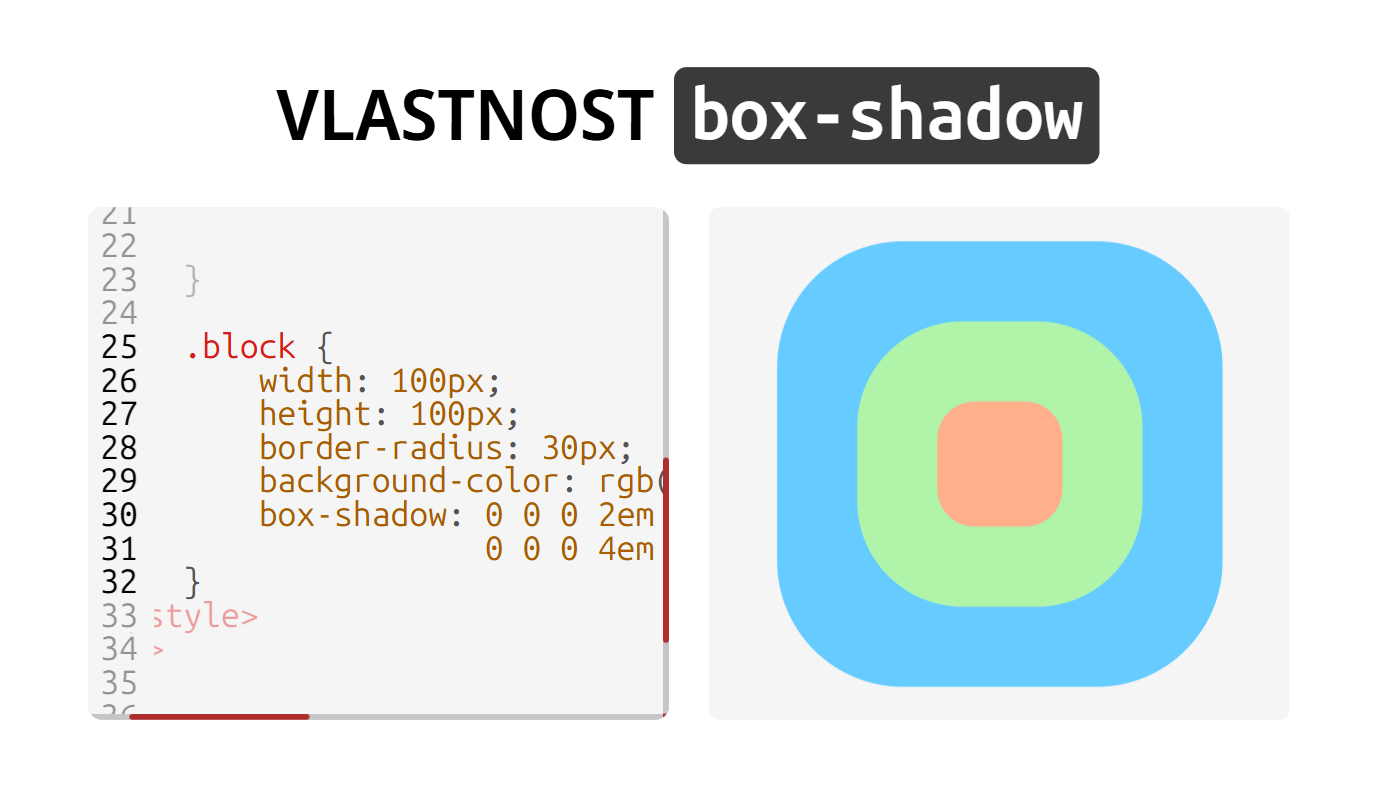
\includegraphics[width=0.9\linewidth]{media/03_analyza/revealjs.png}
    \caption{RevealJS prezentace s rozdělením kódu a výsledku}
    \label{fig:analyza:revealjs-ukazka}
\end{figure}

\subsection{Beamer v \LaTeX}

Beamer je třída v sázecím systému \LaTeX, která se zaměřuje na vytváření snímkových prezentací.
Nejvíce je Beamer společně s \LaTeX~populární v akademickém prostředí zejména z důvodu jednoduchého sázení matematických formulí a zápisu pomocí kódového jazyka, který leccos dovoluje. 

Zápis je ale zároveň to nejvíce nenáviděné na \LaTeX~\cite{latex_reddit}, a to zejména z důvodu kryptických kódových chyb a různých zastaralých zápisů.
Vygenerované prezentace jsou taktéž statické a nedá se v nich dělat jakákoliv interaktivity. 
Výhodou takovéto kódové generace je, že často z jednoho zdrojového kódu -- pro prezentaci -- se dají tvořit taktéž skripta a to tím, že přidáváme takové bloky kódu, které vykreslí právě v jednom nebo v obou módech.

\section{Aplikace na grafickou tvorbu}

Tato sekce se zaměřuje na nástroje, které umožňují snadno a rychle vytvářet vizuálně atraktivní materiály, ať už jde o grafiky, ilustrace, uživatelská rozhraní či jiné kreativní prvky doplňující prezentace a vzdělávací materiály.

\subsection{Canva}\label{text:canva}

Canva je webová platforma pro rychlou a snadnou tvorbu grafických materiálů, jako jsou plakáty, letáky, sociální příspěvky či prezentace, s bohatou nabídkou šablon, fontů a grafických prvků\todo{Zdroj}. 
Hlavní výhody Canvy spočívají v intuitivním uživatelském rozhraní\todo{Zdroj}, obrovské knihovně předpřipravených šablon a prvků, možnosti drag-and-drop úprav a snadné integraci multimédií.

Díky cloudovému prostředí umožňuje Canva týmovou spolupráci\todo{Zdroj}, sdílení souborů v reálném čase a přístup k materiálům odkudkoli, přičemž většina základních funkcí je dostupná zdarma. 

Nevýhodou může být omezenější možnost zcela individuálního designu u některých šablon, menší preciznost u specifických grafických úprav a u pokročilých funkcí potřeba placené verze Canva Pro. 
Přesto je Canva velmi oblíbená pro rychlou tvorbu vizuálně atraktivních materiálů i mezi pedagogy, kteří nepotřebují pokročilé znalosti grafických programů a chtějí rychle připravit poutavé grafické materiály či prezentace.
Čeští pedagogové mají program Canva k dispozici zdarma po ověření\todo{Zdroj}. Tento nástroj je mezi pedagogy velmi oceňován zejména právě pro jeho jednoduchost\todo{Zdroj}.

\subsection{Figma}

Figma je profesionální online nástroj pro design a prototypování uživatelských rozhraní, který se v posledních letech stal standardem v oblasti webového a aplikačního designu\todo{Zdroj}. 
Nabízí vektorový grafický editor, možnost vytvářet interaktivní prototypy a sdílet je v reálném čase s kolegy, což výrazně usnadňuje spolupráci v týmech\todo{Zdroj}. 
Velkou předností Figmy je její cloudové prostředí, ve kterém se změny ukládají automaticky, a každý člen týmu vidí okamžité aktualizace, což zjednodušuje proces zpětné vazby a revizí. 

Nevýhodou může být vyšší křivka učení pro uživatele neznalé profesionálních grafických nástrojů a nutnost stabilního připojení k internetu, aby bylo možné plně využít funkce Figmy. 
Přesto Figma představuje výkonný a flexibilní nástroj, který může pedagogům a školám pomoci při tvorbě interaktivních rozhraní pro studijní materiály, e-learningové platformy či jiné digitální vzdělávací projekty.

\section{Aplikace na tvorbu materiálů}\todo{Celkově k tomuhle dopsat spoustu věcí}

Tato sekce představuje nástroje, jež umožňují připravovat a distribuovat výukové materiály v podobě interaktivních prezentací, kvízů, vizuálních map či jiných vzdělávacích formátů.
Tyto nástroje tedy cílí na velmi podobné cíle, které má i moje budoucí aplikace.
Hlavním cílem těchto aplikací je zefektivnit a zpestřit proces učení, zvýšit zapojení studentů a nabídnout pedagogům možnosti, jak obohatit svou výuku o moderní a atraktivní formy obsahu.

\subsection{Genially}

Genially je online platforma pro tvorbu interaktivních materiálů, prezentací, infografik a dalších multimediálních podkladů, které mohou publikum aktivně zapojit do obsahu.
Platforma je navržena s důrazem na jednoduchost použití, aby byla dostupná jak profesionálům, tak i laikům.

Jednou z klíčových vlastností Genially je možnost rychlého přidávání interaktivních prvků\todo{Zdroj}, jako jsou kvízy, hypertextové odkazy, animace a různorodý multimediální obsah. 
Tyto funkce nejen zvyšují zapojení studentů, ale také podněcují jejich motivaci k učení skrze aktivní interakci s obsahem. 
Tím se platforma stává nejen nástrojem pro prezentaci informací, ale také prostředkem pro výuku založenou na principu konstruktivistické pedagogiky\todo{Zdroj}. 
% Konkrétní příklady interaktivních prvků zahrnují již zmíněné odkazy, kliknutí, řazení, kvízy, interaktivní aplikace uvnitř a mnoho dalšího.

Velkou předností Genially je jeho intuitivní rozhraní a široká škála připravených šablon.
Tyto šablony jsou navrženy s ohledem na vizuální atraktivitu a dynamiku, což umožňuje rychlou tvorbu obsahu bez nutnosti pokročilých grafických znalostí.
Platforma tak poskytuje tvůrcům nástroje, které by jinak vyžadovaly komplexní software a odborné znalosti.

Genially je však placená služba, což může představovat značnou překážku pro vzdělávací instituce a jednotlivce s omezenými finančními zdroji. 
Bezplatná verze nabízí pouze omezenou funkcionalitu a materiály vytvořené v rámci této verze obsahují vodoznak.
Dále je export obsahu možný pouze u placených tarifů, a to v různých formátech, jako jsou PDF nebo HTML. 
Tato omezení mohou snižovat flexibilitu uživatele, který by chtěl svůj obsah sdílet, archivovat offline a nebo celkově více plánovat výuku. 
Zároveň nelze provádět vlastní úpravy kódu ani integrovat komunitní rozšíření, což omezující uživatele, kteří by potřebovali pokročilé nebo zcela unikátní funkce.

Je třeba zmínit, že Genially jako firma je formálně napojena na platformu Canva\todo{Zdroj}, viz kapitola \ref{text:canva}, a tyto dvě služby sdílejí základ vizuálního editoru. 
Tento aspekt zvyšuje celkovou kvalitu uživatelského zážitku, protože editor se vyznačuje vysokou přehledností a snadnou manipulací s obsahem. 
Z tohoto pohledu lze považovat Genially za nástroj, který efektivně staví na osvědčených principech uživatelského designu a zajišťuje širokou dostupnost profesionálních vizuálních standardů.

Na základě vlastních zkušeností jsem využil Genially pro tvorbu několika prezentací a vzdělávacích materiálů. 
Zatímco samotná tvorba byla rychlá a relativně bezproblémová, setkala jsem se s určitými nedostatky, které ztěžovaly optimální využití platformy. 
Jedná se o:\todo{Dopsat}

\begin{itemize}
    \item omezenost obsahu
    \item limitace "klavesnice"
\end{itemize}


\subsection{Mentimeter}

Mentimeter je webová aplikace určená pro interaktivní zapojení publika prostřednictvím online hlasování, dotazníků, kvízů, slovních mraků, průzkumů a anket\todo{Zdroj}. 
Umožňuje učitelům a přednášejícím získávat okamžitou zpětnou vazbu od studentů, což napomáhá identifikovat oblasti nepochopení, zvýšit míru interakce a podporovat aktivní účast na výuce. 

Velkou předností Mentimeteru je jeho uživatelská přívětivost, široká nabídka interaktivních formátů, kompatibilita s mobilními zařízeními a snadná integrace do výukových scénářů, přičemž výsledky lze ihned zobrazit na obrazovce. 
Vzhledem k tomu, že Mentimeter se zaměřuje zejména na interakci a aktivní zapojení publika, nikoliv na obsah samotný, nenabízí mnoho grafických funkcí pro tvorbu složitých nebo vizuálně bohatých materiálů\todo{Zdroj}. 

Stejně jako Genially zde chybí komunitně tvořené rozšíření a detailní možnosti kódových úprav, avšak pokud je cílem zvýšit interaktivitu a okamžitou odezvu od studentů, Mentimeter tento úkol splní velmi dobře.

Mentimeter jsem aplikoval několikrát ve výuce a splnil to, co jsem očekával, a to, že se zvýšila interaktivita ve výukové skupině. 
Velký problémem je opravdu to, že obsah nejde upravovat natolik, aby šlo vytvořit cokoliv. 
V aplikace taktéž velmi chybí grafické možnosti, na jednotlivé snímky lze vložit pouze jeden interaktivní prvek s jednotkami grafických variací.

\subsection{Prezi}

Prezi je prezentační nástroj, který se odlišuje od klasických lineárních prezentací svou nelineární strukturou.
Místo jednotlivých snímků pracuje Prezi s jedním velkým plátnem\todo{Zdroj}, na němž lze rozmístit text, obrázky, videa a další obsah do logických celků, mezi kterými lze dynamicky přecházet pomocí pohyblivých či přibližovacích efektů.
Aplikace je tedy takovou velkou jednou myšlenkovou mapou.
To však omezuje její použití na pouze jeden konkrétní případ způsobu výuky -- obyčejné prezentace zde vypadají velmi zvláštně.

Hlavní předností Prezi je vizuální atraktivita, flexibilita v organizaci obsahu a neobvyklý způsob zobrazení témat, který může pomoci udržet pozornost posluchačů a lépe vyjádřit souvislosti mezi jednotlivými informacemi. 

Nicméně Prezi nenabízí výrazně interaktivní prvky pro zapojení studentů, nepodporuje komunitně tvořená rozšíření a soustředí se především na vizuální aspekt prezentací, nikoliv na interakci či možnost programových úprav.

Prezi jsem se snažil použít, jejich editor je však velmi zvláštní a odbočuje od známých standardů \texttt{UI} a \texttt{UX}.
Prezi je taktéž placená aplikace a omezuje použití jakýchkoliv pokročilých bloků za placenou verzí a tedy použití je prakticky bez toho nemožné.

\section{Sumarizace knihoven a nástrojů}

% Tabulka kde vse vyse uvedene nejak sumarizuji, co chybi

% \begin{table}[h!]
% \centering
% \resizebox{\textwidth}{!}{%
% \begin{tabular}{r|c|c|c|c|c|c|c|c|c|}
% Vlastnost / Služba/knihovna &
%   \cellcolor[HTML]{EFEFEF}Genially &
%   \cellcolor[HTML]{EFEFEF}Mentimeter &
%   \cellcolor[HTML]{EFEFEF}Prezi &
%   \cellcolor[HTML]{EFEFEF}Canva &
%   \cellcolor[HTML]{EFEFEF}Figma &
%   \cellcolor[HTML]{EFEFEF}PowerPoint &
%   \cellcolor[HTML]{EFEFEF}Google Slides &
%   \cellcolor[HTML]{EFEFEF}RevealJS &
%   \cellcolor[HTML]{EFEFEF}Beamer \\ \hline
% \multicolumn{1}{|r|}{\cellcolor[HTML]{EFEFEF}Tvorba prezentací} &
%   \cmark &
%   \xmark &
%   \xmark &
%   \cmark &
%   \cmark &
%   \cmark &
%   \cmark &
%   \cmark &
%   \cmark \\ \hline
% \multicolumn{1}{|r|}{\cellcolor[HTML]{EFEFEF}Tvorba materiálů} &
%   \cmark &
%   \xmark &
%   \xmark &
%   \xmark &
%   \cmark &
%   \xmark &
%   \xmark &
%   \xmark &
%   \xmark \\ \hline
% \multicolumn{1}{|r|}{\cellcolor[HTML]{EFEFEF}Tvorba grafiky} &
%   \cmark &
%   \xmark &
%   \xmark &
%   \xmark &
%   \cmark &
%   \xmark &
%   \xmark &
%   \xmark &
%   \xmark \\ \hline
% \multicolumn{1}{|r|}{\cellcolor[HTML]{EFEFEF}Spolupráce v reálném čase} &
%   \cmark &
%   \cmark &
%   \cmark &
%   \cmark &
%   \cmark &
%   \cmark (web. verze) &
%   \cmark &
%   \xmark &
%   \xmark \\ \hline
% \multicolumn{1}{|r|}{\cellcolor[HTML]{EFEFEF}Způsob zápisu} &
%   GUI &
%   GUI &
%   GUI &
%   GUI &
%   GUI &
%   GUI + XML &
%   GUI &
%   HTML &
%   LaTeX \\ \hline
% \multicolumn{1}{|r|}{\cellcolor[HTML]{EFEFEF}Open-source} &
%   \xmark &
%   \xmark &
%   \xmark &
%   \xmark &
%   \xmark &
%   \xmark &
%   \xmark &
%   \cmark &
%   \cmark \\ \hline
% \multicolumn{1}{|r|}{\cellcolor[HTML]{EFEFEF}Interaktivita} &
%   \cmark &
%   \cmark &
%   \cmark &
%   \xmark &
%   \xmark &
%   \xmark &
%   \xmark &
%   \cmark &
%   \xmark \\ \hline
% \end{tabular}%
% }
% \caption{aaa}
% \label{tab:my-table}
% \end{table}\todo{Dát asi do dvou/tří tabulek?}

Možná už teď více definovat co jsou nutné problémy k vyřešení

\section{Interaktivní prvky}

Podívat se jak fungují různé nástroje pro vzdělávání, interakce, např. hello-algo, kahoot, blooket

\section{Komunitní rozšíření a jejich správa}

Jak to resi google, revealjs ale i neco pokrocilejsiho, hlavne resit bezpecnost

\section{Uživatelé aplikace}

\section{Požadavky}